	
	\section{Contiki als \ac{os} für verteilte Systeme}
	\subsection{\ac{6lowpan} Operating Systems im Vergleich}
	Es gibt mehrere  verschiedene Operating Systems, die einen \ac{6lowpan} Stack beinhalten. Diese Systeme unterstützen meistens die Protokolle, die in einem internetfähigen Gerät benötigt werden. Dadurch hat man ein System, welches die Kommunikation von der \ac{phy}- bis zur Application-Layer gewährleistet.\\
	Operating Systems, die diese Funktionalitäten bieten sind beispielsweise Contiki, TinyOS oder RIOT (Abb. \ref{os6lowpan}). All diese Operating Systems sind unter einer freien Lizenz verfügbar. Die Systeme werden innerhalb einer Github Repository entwickelt. Dies ermöglicht jedem User direkten Zugriff auf den gesamten Quellcode. TinyOS und Contiki sind mit einer BSD-Lizenz lizenziert. Dies bedeutet, dass der Programmierer, wenn er einen Binärcode veröffentlicht, nicht dazu verpflichtet ist auch den Quellcode zu veröffentlichen. Wird jedoch der nicht kompilierte Quellcode veröffentlicht, muss auch Die BSD-Lizenz im Quellcode vorhanden sein. RIOT hingegen ist mit einer GNU Lesser General Public License v2.1 lizensiert. Dies bedeutet, dass die Software in der eigenen Software verwendet und eingebunden werden kann, ohne dass der komplette Quellcode der darauf aufbauenden Software veröffentlicht werden muss. Werden jedoch Teile des lizenzierten Quellcodes verändert, so muss dieser Teil anderen Nutzern zugänglich gemacht werden.\\
	\begin{figure}
		\centering
		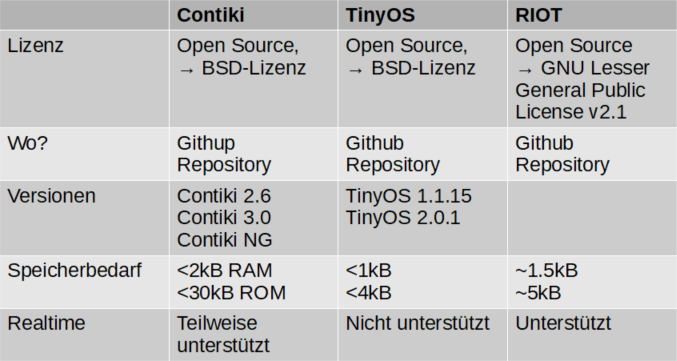
\includegraphics[scale=1]{Grafiken-Julian/OperatingSystemsVergleich.png}
		\caption{Operating Systems mit \ac{6lowpan} Implementierungen}
		\label{os6lowpan}
	\end{figure}
	Da \ac{6lowpan} auf ressourcensparenden Geräten zum Einsatz kommen soll, ist unter anderem auf den Energieverbrauch aber auch auf den Speicherbedarf zu achten. Contiki hat dabei den größten Speicherbedarf von ca. 2kB \ac{ram} und ca. 30kB \ac{rom}. Etwas weniger benötigt RIOT mit 1,5kB \ac{ram} und 5kB \ac{rom}. TinyOS ist in dieser Hinsicht führend mit ca. 1kB \ac{ram} und 4kB \ac{rom}. Nur RIOT ist wirklich Realtime fähig. Contiki unterstützt dies nur teilweise. TinyOS hingegen gar nicht. Da \ac{6lowpan} als Möglichkeit einer Realisierung von IOT gesehen wird, ist die Unterstützung von Realtime wichtig.\\
	Im Zuge der Recherche zu \ac{6lowpan} stellte sich heraus, dass diese Systeme alle noch in der Entwicklungsphase sind. Aufgrund mehrere Implementierungen eines \ac{6lowpan}-Netzwerkes mit Conitki, haben wir uns für dieses Operating System entschieden. Jedoch stellte sich auch hier im Laufe des Projekts heraus, dass die Dokumentation über dieses System und insbesondere auch den Quellcode sehr gering ist. Dies erschwerte die Nutzung des Systems erheblich.\\
	
	Contiki ist ein Open Source System, welches allgemein Low-Power Wireless Standards unterstützt. Contiki besitzt die nötigen Stacks um mithilfe \ac{6lowpan} in einem Netz zu kommunizieren. Contiki unterstützt dabei verschiedene Protokolle in den verschiedenen Layern. Contiki unterstützt beispielsweise \ac{coap} aber auch \ac{http} im Application-Layer. Dadurch kann je nach Anwendung das passende Protokoll gewählt werden. Contiki unterstützt Protokolle wie \ac{ipv6}, \ac{udp}, \ac{tcp}, \ac{6lowpan} und viele weitere.\\
	Contiki selbst bezeichnet sich als „The Open Source Operating System for the Internet of Things“. Zielplattformen von Contiki sind batteriebetriebene Embedded Systems. Dadurch ergeben sich wichtige Anforderungen für das Betriebssystem:
	\begin{itemize}
		\item Speicher\\
		Ressourcenschonende Mikrocontroller besitzen nur wenig Speicher. Deshalb muss auch beim Betriebssystem darauf geachtet werden, dass möglichst wenig Speicher für das Betriebssystem selbst verbraucht wird. Dadurch soll genügend Speicher für die eigentlichen Anwendungsprogramme übrig bleiben.       
		\item Energieverbrauch\\
		\ac{6lowpan} sieht vor, dass ein Mikrocontroller-Knoten mehrere Jahre wartungsfrei von einer Batterie betrieben wird. Deshalb ist es sehr wichtig, dass das Betriebssystem Stromsparmaßnahmen vorsieht, damit solch lange Betriebszeiten mit einer Batterie realisiert werden können. Da \ac{6lowpan}-Knoten oft Sensoren sind, können deshalb nicht benötigte Peripherien des Mikrocontrollers oder des Sensors abgeschaltet werden. Als größter Energieverbraucher gilt jedoch das Funkmodul. Contiki besitzt deshalb ein System, welches das Funkmodul möglichst effizient an- bzw. abschaltet.
	\end{itemize}
	
	Contiki ist deshalb auch nur für bestimmte Plattformen und Prozessoren verfügbar. Contiki unterstützt beispielsweise die MSP430x-Serie oder verschiedene AVR Mikrocontroller jeweils in Verbindung mit einem Funkmodul. Im vorliegenden Projekt wird das "'CC1310 Launchpad"' von Texas Instruments als Plattform verwendet. Im CC1310 Launchpad sind Prozessor und Funkmodul in einem Chip kombiniert, wodurch es möglich ist Contiki \ac{os} ohne zusätzlichen Peripherien(andere Boards) zu nutzen.
	
	\subsection{Protokollstacks}
	Contiki unterstützt den kompletten Protokollstack vom Physical Layer bis hin zum Application Layer. Contiki bietet dabei noch die Möglichkeit in den verschieden Layers verschiedene Protokolle zu verwenden. Dadurch kann Contiki viele verschiedene Einsatzgebiete haben, da je nach Anwendung das benötigte Protokoll ausgewählt werden kann. Abbildung \ref{protokollstack} zeigt dabei verschiedene Möglichkeiten den Protokollstack zu implementieren.\\
	\begin{figure}
		\centering
		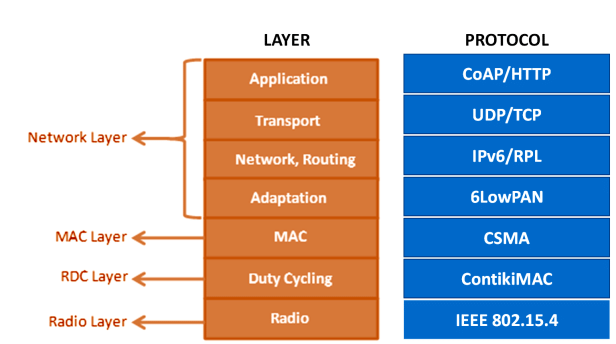
\includegraphics[scale=0.5]{Grafiken-Julian/ProtokollStacksContiki.png}
		\caption{Protkollstack des Contiki Operating Systems, \cite{contikiprotokollstack}}
		\label{protokollstack}
	\end{figure}
	Auf den unteren Layern (\ac{phy}) teilt sich der Stack von Contiki in zwei Layer auf. Zum einen in den \ac{15.4} Stack und den ContikiMAC Stack, der zwischen \ac{phy}- und \ac{mac}-Layer liegt. Der ContikiMAC Layer nimmt dabei eine ganz besondere Funktion ein. Der ContikiMAC ist unter anderem dafür verantwortlich, dass das Funkmodul möglichst wenig aktiv ist. Das Funkmodul ist im gesamten System der größte Energieverbraucher und wird deshalb nur sequenziell an- und abgeschaltet. Abbildung \ref{ContikiMAC} zeigt die verschiedenen Möglichkeiten wie ein Paket mit und ohne Phasenoptimierung verschickt beziehungsweise empfangen werden kann. Im Falle ohne Phasen-Optimierung, sendet der Sender so lange (mit der Bedingung, dass das der Sendezeitraum nicht eingeschränkt ist), bis der Sender ein \ac{ack}-Paket vom Empfänger erhält. Der Energieverbrauch ist in diesem Fall unnötig hoch, da ein Node so programmiert ist, dass er nur in bestimmten Zeitabschnitten eine Funkkommunikation aufbaut. Der Sender kann deshalb, ausgehend von früheren Kommunikationen zum Node speichern, wann ein Node zur Kommunikation bereit ist. Durch dieses Verfahren wird der Energieverbrauch erheblich gesenkt. Der ContikiMAC trägt damit hauptsächlich dazu bei, dass der Stromverbrauch der Nodes gering gehalten werden kann. Der \ac{mac} Layer in Contiki benutzt auch \ac{csmaca}. Dadurch wird sichergestellt, dass mehrere Nodes nicht gleichzeitig senden und Pakete über Funk korrekt empfangen werden. \\
	\begin{figure}
		\centering
		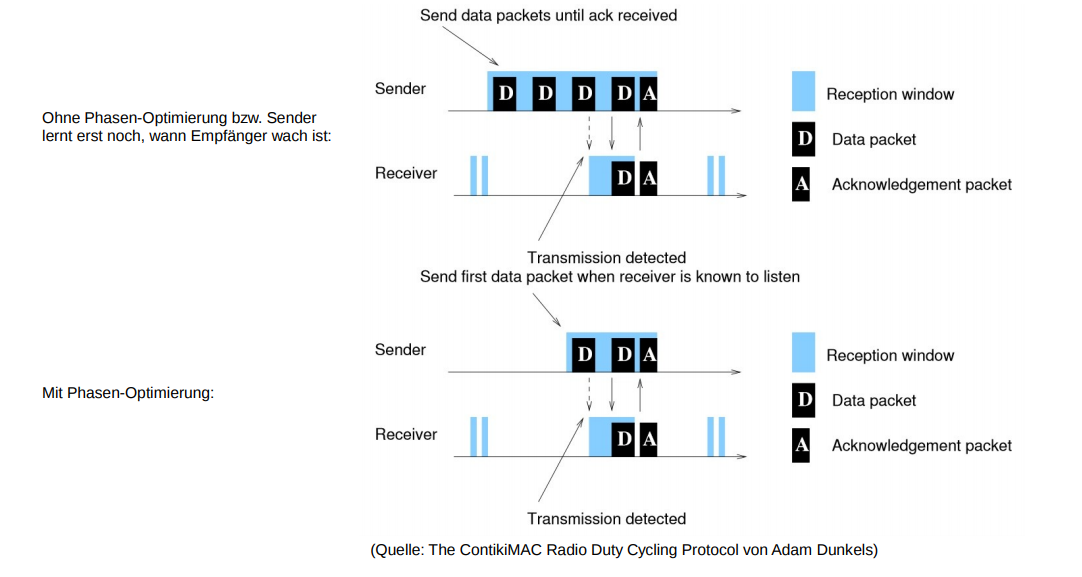
\includegraphics[scale=0.5]{Grafiken-Julian/ContikiMAC.png}
		\caption{Funktionsweise des ContikiMAC's mit Phasenoptimierung, \cite{dunkelsmac}}
		\label{ContikiMAC}
	\end{figure}
	Nach dem \ac{csmaca} Stack folgt der \ac{6lowpan} Stack, der als Adaptionslayer zwischen \ac{ipv6} und dem \ac{mac}-Layer dient. Mithilfe des \ac{6lowpan} Protokoll wird der Header der überliegenden Layern erheblich verkleinert. Durch das \ac{6lowpan} Protokoll kann der Header eines \ac{ipv6} Pakets so verkleinert werden, dass die maximal zulässige Größe eines \ac{15.4} Pakets eingehalten werden kann. Deshalb ermöglicht dieses Protokoll erst die Nutzung des \ac{15.4} Protokolls und damit eine energiesparende Funkübertragung.\\
	Im Network Layer bietet Contiki die Nutzung von \ac{ipv6} und \ac{rpl}.\\
	Auf der Transportschicht kann man sich für \ac{tcp} oder \ac{udp} entscheiden. \ac{tcp} macht jedoch in Kombination mit \ac{6lowpan} und \ac{15.4} wenig Sinn, da \ac{tcp} einen noch größeren Header besitzt als \ac{udp}. Da \ac{tcp} nicht komprimiert wird, ist dies allein aufgrund der Headergröße nicht möglich. \ac{tcp} ist ein verbindungsorientiertes Protokoll und bietet deshalb mehr Sicherheit, dass Pakete richtig (in der richtigen Reihenfolge, keine Bitfehler...) empfangen werden. Da mit \ac{6lowpan} ein Sensornetzwerk betrieben werden soll, wo die Sensoren beispielsweise nur jede Minute einen neuen Wert liefern, kann es auch vernachlässigt werden, wenn einzelne Nachrichten falsch oder gar nicht ankommen. Da \ac{udp} auf bestimmte Sachen aus dem \ac{tcp} Protokoll verzichtet, wird \ac{udp} allgemein als die unkompliziertere und schnellere Verbindung angesehen.\\
	Auf der Applikationsschicht kann zwischen \ac{coap} und \ac{http} entschieden werden. Wie bei \ac{tcp} und \ac{udp}, ist \ac{coap} im Vergleich zu \ac{http} das schlankere Protokoll und bietet sich deshalb auch für ein \ac{6lowpan} Netzwerk an.\\
	
	Contiki \ac{os} hat den Vorteil, dass es viele Protokollstacks beinhaltet. Dadurch kann individuell an die benötigten Strukturen der Anwendung der Stack "'zusammengesucht"' werden. Hauptgebiet von Contiki \ac{os} bleiben jedoch vorerst \ac{6lowpan} Netzwerke.
	
	\subsection{Prozess}
	Contiki \ac{os} basiert auf verschiedenen Prozessen. Diese Prozesse werden eventbasiert aufgerufen. In Contiki gibt es grundsäzlich zwei verschiedene Arten wie ein Prozess ausgeführt werden kann.
	\begin{itemize}
		\item Kooperativ\\
		Kooperative Prozessen werden nacheinander aufgerufen. Sobald ein Prozess beendet wurde, kann der nächste Prozess gestartet werden. Der Aufbau der Prozesse darf jedoch nicht direkt mit einem RTOS verglichen werden, da ein Prozess nicht sequentiell aufgerufen wird, sondern nur dann wenn dieser Prozess auch ausgelöst (Event) wurde. Ein kooperativer Prozess unterbricht nie einen laufenden Prozess. Kooperative Prozessen sind Bestandteil der ganz normalen Programmausführung.
		\item Präventiv\\
		Ein präventiver Prozess ist vergleichbar mit einem Interrupt. Ein präventiver Prozess unterbricht den laufenden Prozess und wird dann ausgeführt. Nach Beenden des präventiven Prozesses springt das \ac{os} in den unterbrochenen Prozess zurück. Dieser kann anschließend fortgeführt werden. 
	\end{itemize}
	
	Contiki \ac{os} ist grundsätzlich so aufgebaut, dass es viele kooperative Prozesse gibt und nur einzelne präventive Prozesse, die den "'normalen"' Programmablauf unterbrechen. Der Programmablauf wird mithilfe einer Eventqueue im Kernel geregelt. Die Eventqueue wird nach dem Prinzip eines \ac{fifo} abgearbeitet. Ist die Eventqueue leer werden deshalb auch so lange keine Prozesse mehr ausgeführt bis ein neuer Event in die Eventqueue geschrieben wird.
	
	Den Quellcode, wie ein Prozess deklariert wird, zeigt Abbildung \ref{ContikiProzess}. Der Name des Prozesses wird mit PROCESS\_THREAD("'Prozessname"') festgelegt. Der eigentliche Prozess wird dann innerhalb PROCESS\_BEGIN() und PROCESS\_END() definiert. PROCESS\_BEGIN(), PROCESS\_END() und PROCESS\_THREAD() sind lediglich Defines, die die Programmierung von Prozessen vereinfachen sollen. Die Defines stellen dabei in Kombination eine Switch Case Abfrage dar. Mithilfe dieser Struktur wird der ganze Prozessablauf in Contiki \ac{os} geregelt.
	\begin{figure}
		\centering
		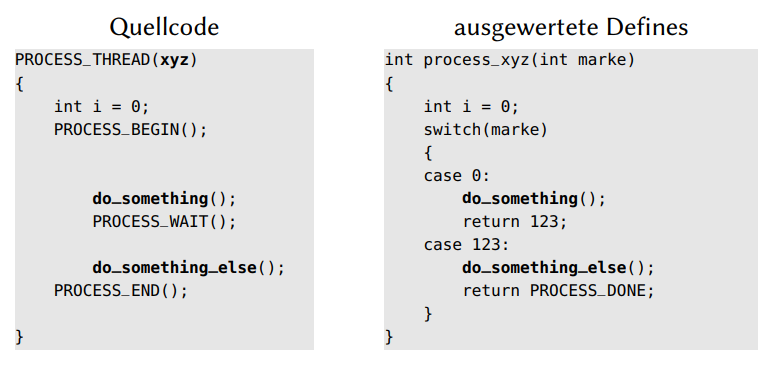
\includegraphics[scale=0.5]{Grafiken-Julian/Contiki_Prozess.png}
		\caption{Aufbau eines Contiki-Prozess, \cite[S.9]{ausgewertetedefines}}
		\label{ContikiProzess}
	\end{figure}
	Diese Defines, die den Code vereinfachen sollen bezeichnet man in Contiki als Protothreads. Um einen Prozess zu strukturieren bietet Contiki \ac{os} mehrere solcher Protothreads an. Die in Contiki \ac{os} vorhanden Protothreads sind:
	
	\begin{itemize}
		\item PROCESS\_BEGIN()\\
		Mit PROCESS\_BEGIN wird der Anfang eines Prozesses deklariert. Der eigentliche Code des Prozesses startet nach PROCESS\_BEGIN().
		\item PROCESS\_END\\
		Mit PROCESS\_END() wird das Ende eines Prozesses deklariert. PROCESS\_BEGIN() und PROCESS\_END() müssen in jedem Prozess angegeben sein. Diese beiden Defines deklarieren den Programmcode des Prozesses.
		\item PROCESS\_EXIT()\\
		Mit PROCESS\_EXIT() wird ein der Prozess verlassen. Der Unterschied zwischen PROCESS\_END() und PROCESS\_EXIT() liegt darin, dass das Define PROCESS\_END() in jeder Prozessdeklarierung enthalten sein muss. PROCESS\_EXIT() kann dann zum Beispiel in einem Unterpfad des Codes verwendet werden um den Prozess zu beenden.
		\item PROCESS\_WAIT\_EVENT\\
		Mit PROCESS\_WAIT\_EVENT wird der Prozess solange pausiert, bis irgendein Event auftritt. Während der Prozess auf einen Event wartet, können andere Prozesse ausgeführt werden. Allerdings löst dieser Event den Prozess erst aus, wenn der auslösende Event durch die Eventqueue zum Kernel gelangt ist.
		\item PROCESS\_YIELD()\\
		Mit PROCESS\_YIELD() wird wie bei PROCESS\_WAIT\_EVENT() der Prozess solange pausiert bis ein Event auftritt.
		\item PROCESS\_WAIT\_EVENT\_UNTIL()\\
		Mit PROCESS\_WAIT\_EVENT\_UNTIL() wird der Prozess nur ausgeführt, wenn ein bestimmter Event ausgelöst wurde. Der nachfolgende Code wird also nur unter bestimmten Eventbedingungen ausgeführt.
		\item PROCESS\_WAIT\_UNTIL()\\
		Mit PROCESS\_WAIT\_UNTIL() wird auf irgendeine Bedingung gewartet. Allerdings besteht bei diesem Protothread die Möglichkeit, dass der Prozessspeicher nicht abgegeben wird. Der Prozess befindet sich dann möglicherweise in einer Endlosschleife und das Programm wird nicht weiter ausgeführt.
		\item PROCESS\_PAUSE()\\
		Mit PROCESS\_PAUSE() wird der Prozess kurz pausiert und ein anderer Prozess kann ausgeführt werden.
	\end{itemize}
	Protothreads die auf einen Event warten, bis dieser ausgelöst wurde, bieten die Möglichkeit den Programmablauf gut zu strukturieren. Wichtig ist dabei, dass andere Prozesse ausgeführt werden können während ein anderer Prozess auf einen Event wartet.
	
	\subsection{Events}
	Contiki \ac{os} ist ein eventbasiertes Betriebssystem. Events nehmen bei Contiki deshalb eine wichtige Rolle ein. Ohne Events wird der Programmcode von Contiki nur einmal ausgeführt. Erst durch Events wird der Programmcode flexibel. Contiki \ac{os} besitzt deshalb drei verschiedene Arten von Events:
	
	\subsubsection{Asynchroner Event}
	Ein asynchroner Event wird durch den Aufruf von process\_post() aufgerufen. Parameter die dabei übergeben werden müssen, sind der Pointer des Prozesses, welcher Event Identifier ausgelöst werden soll und eine optionale Nachricht, die mitgesendet werden kann. In der Nachricht werden hauptsächlich Daten mitübertragen, die ausgewertet oder bearbeitet werden sollen. Abbildung \ref{BeispielProgramm} zeigt ein Beispielcode, wie ein Event angelegt und ausgelöst werden kann. Außerdem wird ein PROCESS\_EVENT\_TIMER Event abgearbeitet.\\
	Ein asynchroner Event wird nicht sofort ausgeführt wenn er ausgelöst wurde. Mit process\_post() wird der Event in eine Eventqueue hineingeschrieben. Diese Eventqueue wird vom Kernel abgearbeitet. Die Eventqueue wird nach dem Prinzip eines \ac{fifo}s abgearbeitet. 
	
	\begin{figure}
		\centering
		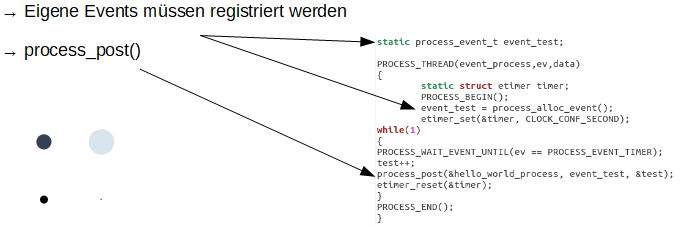
\includegraphics[scale=0.8]{Grafiken-Julian/ContikiEventsCodebeispiel.png}
		\caption{Beispielprogramm mit auslösen eines Events}
		\label{BeispielProgramm}
	\end{figure}
	
	\subsubsection{Synchroner Event}
	Ein synchroner Event ist vergleichbar mit einem Funktionsaufruf in C. Bei diesem Event wird der Prozess innerhalb des anderen Prozesses aufgerufen. Der aufrufende Prozess ist dann eine Ebene über dem aufgerufenen Prozess. Nachdem der aufgerufene Prozess beendet wurde wird der ursprüngliche Prozess weiter ausgeführt. Eine solcher Event wird mit process\_post\_synch() ausgelöst. Wie bei einem asynchronen Prozess werden der Funktion die Parameter des Pointer des Prozesses der aufgerufen werden soll, welcher Event Identifier ausgelöst wird und eine Nachricht übergeben. Der aufgerufen Prozess kann dabei jedoch nicht unterscheiden, ob er von einem asynchronen oder einem synchronen Event ausgelöst wurde.
	\subsubsection{Polling Event}
	Ein poll Event entspricht einem normalen Interrupt. Das heißt, der Event wird sofort ausgeführt. Der laufende Prozess wird dann unterbrochen und die Pollingroutine wird ausgeführt. Diese Event-Funktion ist dann wichtig, wenn zeitkritische Aufgaben (Bsp: Empfang Daten) ausgeführt werden müssen. Ein poll Event wird mit der Funktion process\_poll() ausgelöst. Im Unterschied zu asynchronem und synchronem Event wird lediglich der Prozess anhand seines Pointers aufgerufen. Es wird kein spezieller Event Identifier ausgelöst und es werden keine Nachrichten übermittelt.\\
	
	Alle Arten von Events werden bei Contiki \ac{os} öfters genutzt. Der Programmablauf wird hauptsächlich mit asynchronen Events geregelt. Deshalb nehmen diese Events eine besondere Stellung bei Contiki ein. Abbildung \ref{EventsContiki} zeigt Quellcode, wie die verschiedenen Arten von Events ausgelöst werden können.\\
	Conitiki \ac{os} bietet dem Programmierer 127 frei nutzbare Event Identifiers an. Der Programmierer hat dadurch die Möglichkeit eigene Events zu erstellen, die in seinem Programm gebraucht werden. Contiki hat darüber hinaus acht für den Kernel reservierte Event Identifier:
	\begin{itemize}
		\item PROCESS\_EVENT\_INIT\\
		Dieser Event Identifier wird dem Prozess bei Start von Contiki \ac{os} gesendet
		\item PROCESS\_EVENT\_POLL\\
		Dieser Event Identifier erhält ein Prozess der mit einem poll Event asugelöst wurde.
		\item PROCESS\_EVENT\_EXIT\\
		Diesr Event Identifier wird an einem Prozess gesendet, der vom Kernel beendet wurde. Anschließend wird der vom Prozess benötigte Speicherbereich wieder freigegeben.
		\item PROCESS\_EVENT\_CONTINUE\\
		Diesen Event Identifier erhält ein Prozess, der in einer PROCESS\_YIELD() Operation wartet. Anschließend wird der Prozess weiter ausgeführt.
		\item PROCESS\_EVENT\_MSG\\
		Dieser Event Identifier wird einem Prozess gesendet, wenn eine Kommunikations-Nachricht empfangen wurde. Typischerweise verwendet der IP Stack diesen Identifier um einen anderen Prozess zu informieren, dass eine Nachricht empfangen wurde.
		\item PROCESS\_EVENT\_EXITED\\
		Dieser Identifier wird an alle Prozesse gesendet. Der Event Identifier tritt auf, wenn ein Prozess beendet wurde. Der Kernel informiert damit die übrigen Prozesse, dass ein bestimmter Prozess nicht mehr existiert. Die übrigen Prozesse können dann belegten Speicher des beendeten Prozess im eigenen Prozess freigeben.
		\item PROCESS\_EVENT\_TIMER\\
		Dieser Identifier wird ausgelöst, wenn ein Eventtimer (etimer) abgelaufen ist.
	\end{itemize}	
	Die genannten Event Identifiers werden hauptsächlich für die interne Regelung von Prozessen genutzt. Ein üblicher Programmierer kommt hauptsächlich mit dem PROCESS\_EVENT\_TIMER Event in Kontakt. Die anderen Kernel-Events werden vom Kernel unbemerkt erzeugt und von den Prozessen verarbeitet, sodass der Programmierer dies nicht bemerkt.
	
	\subsection{Prozess Scheduler}
	Der Prozess Scheduler in Contiki regelt den gesamten Programmablauf. Er ist dafür verantwortlich, dass alle Events den richtigen Prozess erreichen. Dabei sorgt er auch dafür, dass der Datenfluss, der mit einem Event einhergeht reibungslos verläuft. Der Prozess Scheduler ist auch welcher, der das komplette Programm startet.\\ 
	Um ein Prozess zu starten, ruft er die Funktion process\_start() auf. Diese Funktion sendet an den aufgerufenem Prozess den PROCESS\_EVENT\_INIT Event Identifier. Daraufhin startet der Prozess(vgl. Abbildung \ref{EventsContiki}). In Contiki selbst wird dies oft direkt bei der Initialisierung gemacht. Der Aufruf lautet dabei AUTOSTART\_PROCESS(), wobei die Parameter der Funktion die einzelnen Adresspointer auf die einzelnen Prozesse sind. Üblicherweise beendet sich der Prozess irgendwann wieder von selbst mit PROCESS\_EXIT() oder PROCESS\_END(). Allerdings besitzt der Prozess Scheduler die Möglichkeit einen Prozess mit proccess\_exit() von außen zu beenden. Dann werden wiederum die belegten Speicher des Prozesses freigegeben. Der Prozess Scheduler ist dabei auch jener, der die anderen Prozesse informiert, dass ein anderer Prozess beendet wurde.
	\begin{figure}
		\centering
		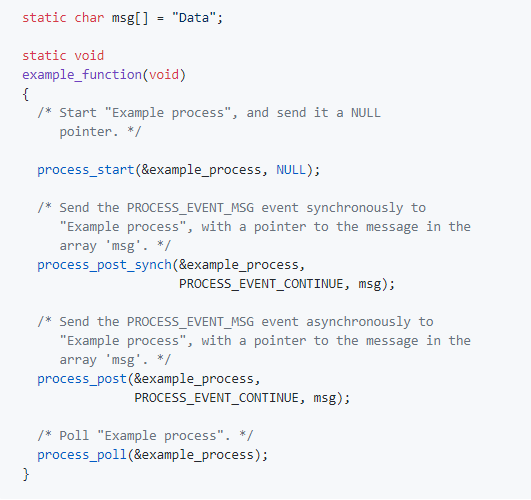
\includegraphics[scale=0.5]{Grafiken-Julian/ContikiEvents.png}
		\caption{Codebeispiel: Auslösen verschiedener Eventarten in Contiki \ac{os}, \cite{codebesipiel}}
		\label{EventsContiki}
	\end{figure}
	\subsection{Contiki Makefile und kompilieren eines Projekts}
	Um ein Contiki \ac{os} Projekt kompilieren zu können, müssen im Projektordner mit dem Programmcode noch weitere Files vorliegen. Ohne das Makefile wird der Programmcode nicht kompiliert. Im Makefile stehen Information für den Compiler bezüglich Projektname, wo Headerdateien zu finden sind und optionale  Defines, um Code flexibel einbinden zu können oder auszuschließen. Ein weiteres wichtiges File ist das Makefile.target, welches ebenfalls optional ist. Wird das Makefile.target nicht erstellt, muss das Target dann dem Compiler vor dem kompilieren angegeben werden. In Instant Contiki wird das Kompilieren mit dem Terminal erledigt. Ein beispielhafter Befehl, wie ein Quellcode kompiliert werden kann, zeigt Abbildung \ref{Makefile&Kompilieren}. \\
	Contiki \ac{os} ist so gestaltet, dass es für verschiedene Plattformen (Prozessoren, Boards) bereits fertige Implementierungen gibt. Deshalb muss immer eine Target angegeben werden. Das hier vorliegende Beispiel soll für das CC1310 Launchpad von Texas Instruments kompiliert werden. Das Target ist deshalb "'srf06-cc26xx"' und das benutzte Board ist das CC1310 Launchpad von Texas Instruments. hello-world.bin in Abbildung \ref{Makefile&Kompilieren} steht dafür, dass der Quellcode in Binärdateien kompiliert werden soll.
	\begin{figure}
		\centering
		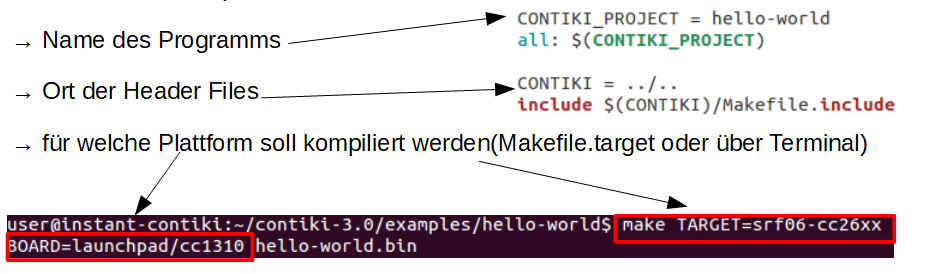
\includegraphics[scale=0.5]{Grafiken-Julian/MakefileKompilieren.png}
		\caption{Erzeugen von Binärdateien mithilfe des Terminals in Instant Contiki}
		\label{Makefile&Kompilieren}
	\end{figure}
	\subsubsection{CC1310 Launchpad und dessen Konfigurationsdateien in Contiki \ac{os}}
	Contiki \ac{os} besitzt für eine Plattform bereits vordefiniert, welche Schnittstellen das Board oder der Prozessor besitzt. Diese Definitionen werden beim Kompilieren eines Projektes verwendet. Die Prozessor spezifischen Einstellungen befinden sich dabei im Conitki-conf.h File. In Contiki-conf.h wird beispielsweise definiert mit welcher Baudrate eine UART-Schnittstelle arbeitet oder bezogen auf \ac{6lowpan}, welche Kompressionsmethode und ab welcher Payload eine Fragmentierung der Pakete vorgenommen werden soll (vgl. Abbildung \ref{Contiki-conf}).\\
	Zusätzlich zum Contiki-conf.h File kann ein zusätzliches projektspezifisches Konfigurationsfile (project-conf.h) angelegt werden. Im project-conf.h File können vorab Einstellungen vorgenommen werden, die  beispielsweise den Stackaufbau betreffen.
	\begin{figure}
		\centering
		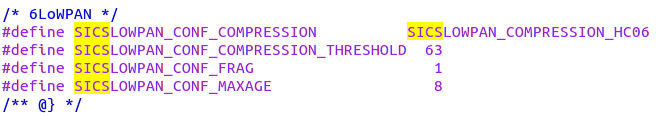
\includegraphics[scale=0.5]{Grafiken-Julian/Contiki_conf.png}
		\caption{Codeauszug des Contiki-conf.h File der srf06-cc26xx Plattform}
		\label{Contiki-conf}
	\end{figure}
	Das board.h File beinhaltet Definitionen bezüglich Pinbelegung (bsp: Pins die an einen Button angeschlossen sind). Contiki hat dabei bereits vordefinierte Defines für Buttons, sodass der Programmierer theoretisch nicht mal wissen muss, an welchen Pin ein Button oder eine Peripherie angeschlossen ist. Abbildung \ref{Boardfiles} zeigt beispielhaft einen Codeauszug aus dem board.h File des CC1310 Launchpads. Die Buttons werden hier dem Pin zugeordnet. Dadurch kann Code leicht auf andere Boards importiert werden ohne den kompletten Code an die neue Plattform anpassen zu müssen. Contiki \ac{os} ist deshalb sehr flexibel für verschieden Plattformen einsetzbar.\\
	\begin{figure}
		\centering
		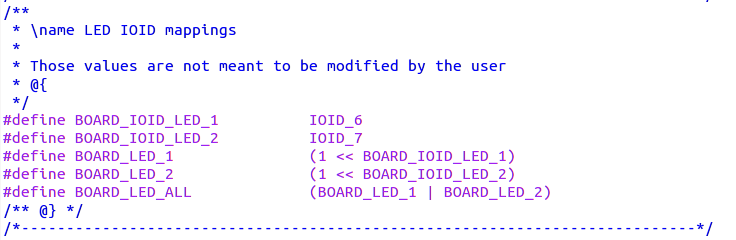
\includegraphics[scale=0.5]{Grafiken-Julian/Boardfiles.png}
		\caption{Codeauszug des board.h File des CC1310 Launchpad in Contiki}
		\label{Boardfiles}
	\end{figure}
	Das in diesem Projekt verwendete Board ist das CC1310 Launchpad. Das Launchpad kann direkt als Funkmodul verwendet werden, da eine PCB Antenne auf dem Launchpad vorhanden ist. Außerdem besitzt es zwei Buttons, die als externe Interrupts verwendet werden können. Das CC1310 Launchpad hat den CC1310 Mikrocontroller verbaut. Dieser besteht aus zwei verschiedenen Prozessoren. Zum einen aus einem ARM Cortex-M3 und einem ARM Cortex-M0. Der ARM Cortex-M3 ist die Haupt-CPU. An ihm sind die ganzen Peripherien (UART, I2C, Timer...) angeschlossen. Der ARM Cortex-M3 regelt die nicht funkbasierte Kommunikation und andere Programmstrukturen. Der zusätzliche ARM Cortex-M0 ist nur für die Funkkommunikation zuständig und um die Daten zu senden oder zu empfangen. Der ARM Cortex-M0 erledigt die unteren Schichten im \ac{osi} Schichtenmodell, wobei der ARM Cortex-M3 für die höherliegenden Schichten zuständig ist.
	\subsection{Elementare Funktionen für die Funkübertragung und den Funkempfang in Contiki \ac{os}}
	Zwei elementare Funktionen in Contiki sind udp\_packet\_send() und der Prozess der ausgeführt wird, wenn ein Paket empfangen wird. Dabei wird oft der tcpip\_event des tcpip.c Files ausgelöst.
	
	
	\begin{itemize}
		\item Paket senden\\
		Abbildung \ref{SendPacket} zeigt beispielhaft einen Sendevorgang eines \ac{udp} Pakets. Generell ist der interne Funktionsablauf bei Aufrufs eines send Request immer ähnlich. Unterschied ist dann, dass unterschiedliche Header verwendet werden. Der grundsätzliche Programmablauf beim Senden eines Pakets ist meist ähnlich.\\
		Ruft ein Programmierer im Programm die Funktion uip\_udp\_packet\_send() (oder ähnlich) auf, so wird mit dem übergeben Parameter die Payload gesetzt(buffer). Daraufhin wird intern eine weitere Funktion (bsp: uip\_process())aufgerufen. In dieser Funktion werden die nötigen UDP Header des Pakets erstellt und der Payload hinzugefügt. In der Folge wird in der xx\_udp\_packet\_send() die Funktion tcpip\_ipv6\_output() (tcpip.c) aufgerufen. Diese Funktion erstellt den \ac{ipv6} Header und durch den Aufruf der output() Funktion aus der sicslowpan.c Datei werden die Headerkomprimierung und Fragmentierung vorgenommen. Die output() Funktion ruft im Programmverlauf die Funktion send\_packet() (sicslowpan.c) auf. Diese leitet eine Anfrage über die Funktion siclowmac\_dataRequest() an die sicslowmac.c Datei, welche das fertige Paket an das Funkmodul weiterleitet, wo es dann letztendlich verschickt wird. Das Seqenzdiagramm in Abbildung \ref{SendPacket} soll diesen Vorgang veranschaulichen.
		\begin{figure}
			\centering
			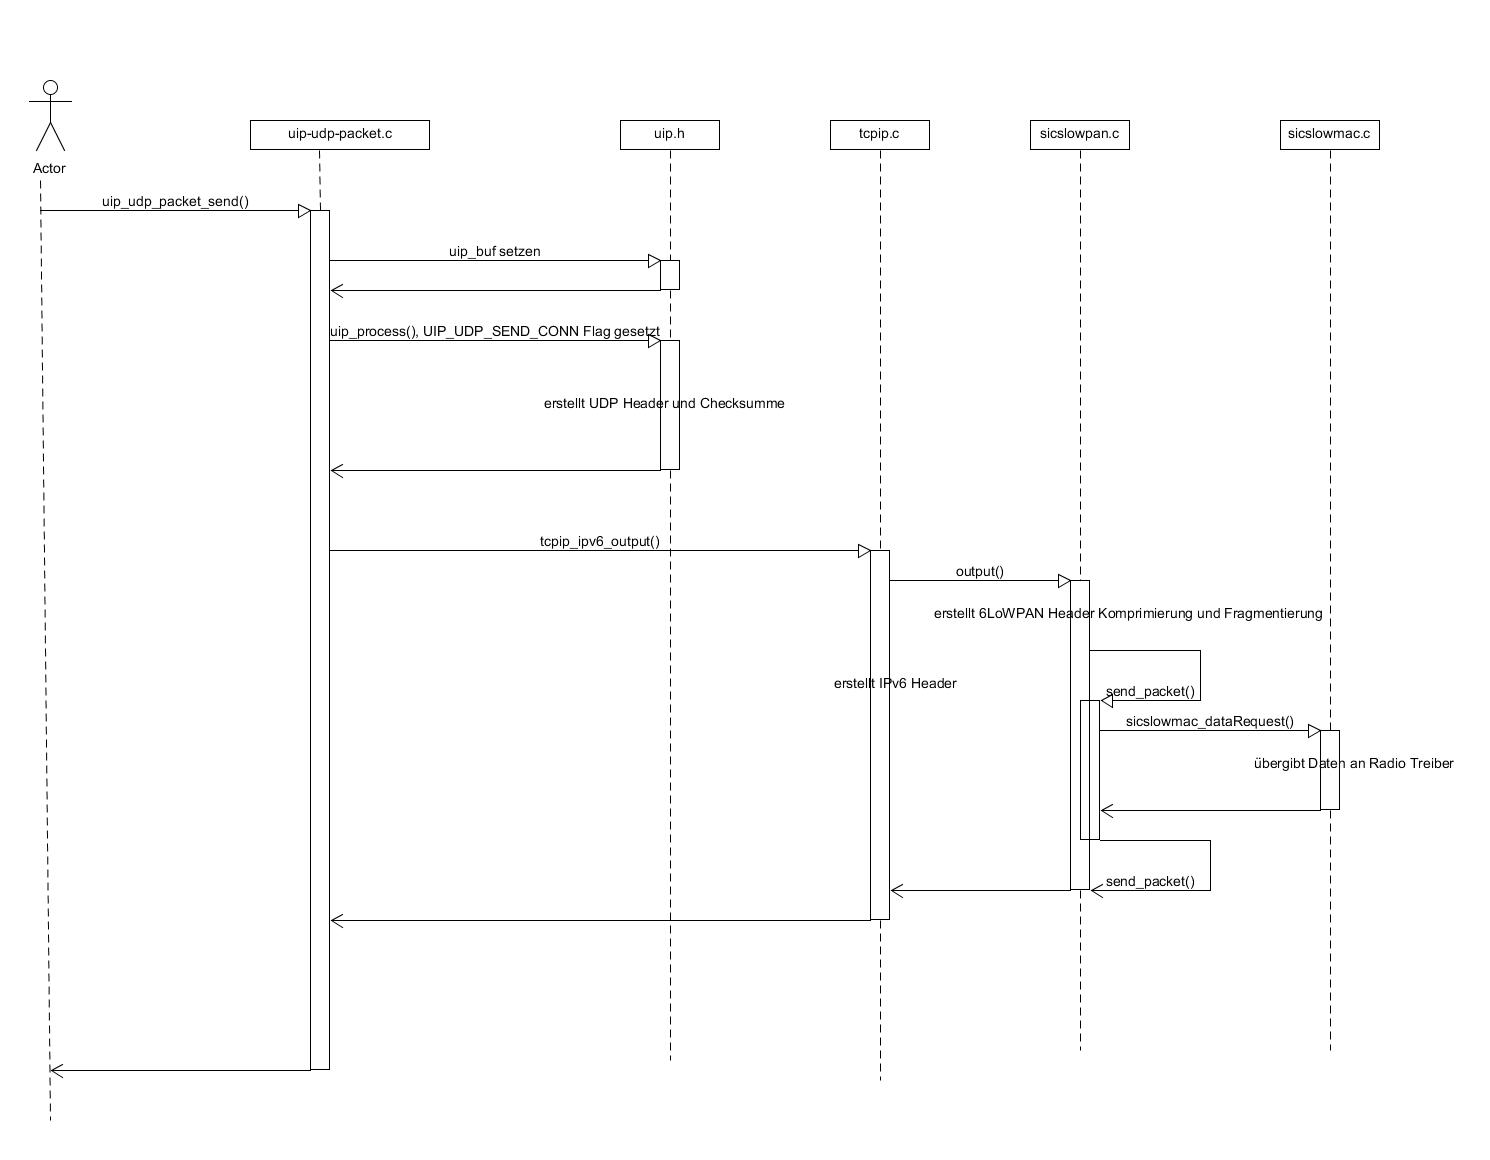
\includegraphics[scale=0.33]{Grafiken-Julian/SendPacket.jpg}
			\caption{Sequenzdiagramm des Funktionsaufruf uip\_udp\_packet\_send() nach nach \cite{sendreceive}}
			\label{SendPacket}
		\end{figure}
		\item Paket empfangen\\
		Abbildung \ref{ReceivePacket} zeigt beispielhaft den Programmablauf bei Empfang eines Pakets. Generell ist der interne Funktionsablauf bei Empfang eines Pakets immer gleich. Wie das Paket weiter verarbeitet wird, entscheidet ein anderer Prozess innerhalb des Ablaufs.\\
		Wird ein Paket empfangen leitet das Funkmodul diese Daten an die sicslowmac\_dataIndication() (siclowmac.c) weiter. Diese Funktion speichert die ankommenden Daten in den Paketbuffer der paketbuf.c Datei. Ist ein Paket komplett empfangen wird mithilfe der Datenlänge der Headerbereich von der Payload mit der Funktion paketbuf\_set\_datalen() getrennt. Anschließen werden die einzelne Fragmente mit der Funktion input() (siclowpan.c) wieder zusammengesetzt und der \ac{ipv6} Header wird wieder dekomprimiert. Im Verlauf dieser Funktion wird dann auch ein synchroner Event an den tcpip\_process() (tcpip.c) ausgelöst. Innerhalb dieser Funktion werden weitere Schritte vorgenommen, um das Paket und die darin enthaltene Payload zu verwerten. Letztendlich wird in der Funktion uip\_process() die zuständige Callback Funktion des Programmierers aufgerufen.\\
		Der gesamte Programmablauf soll Abbildung \ref{ReceivePacket} verdeutlichen.
		\begin{figure}
			\centering
			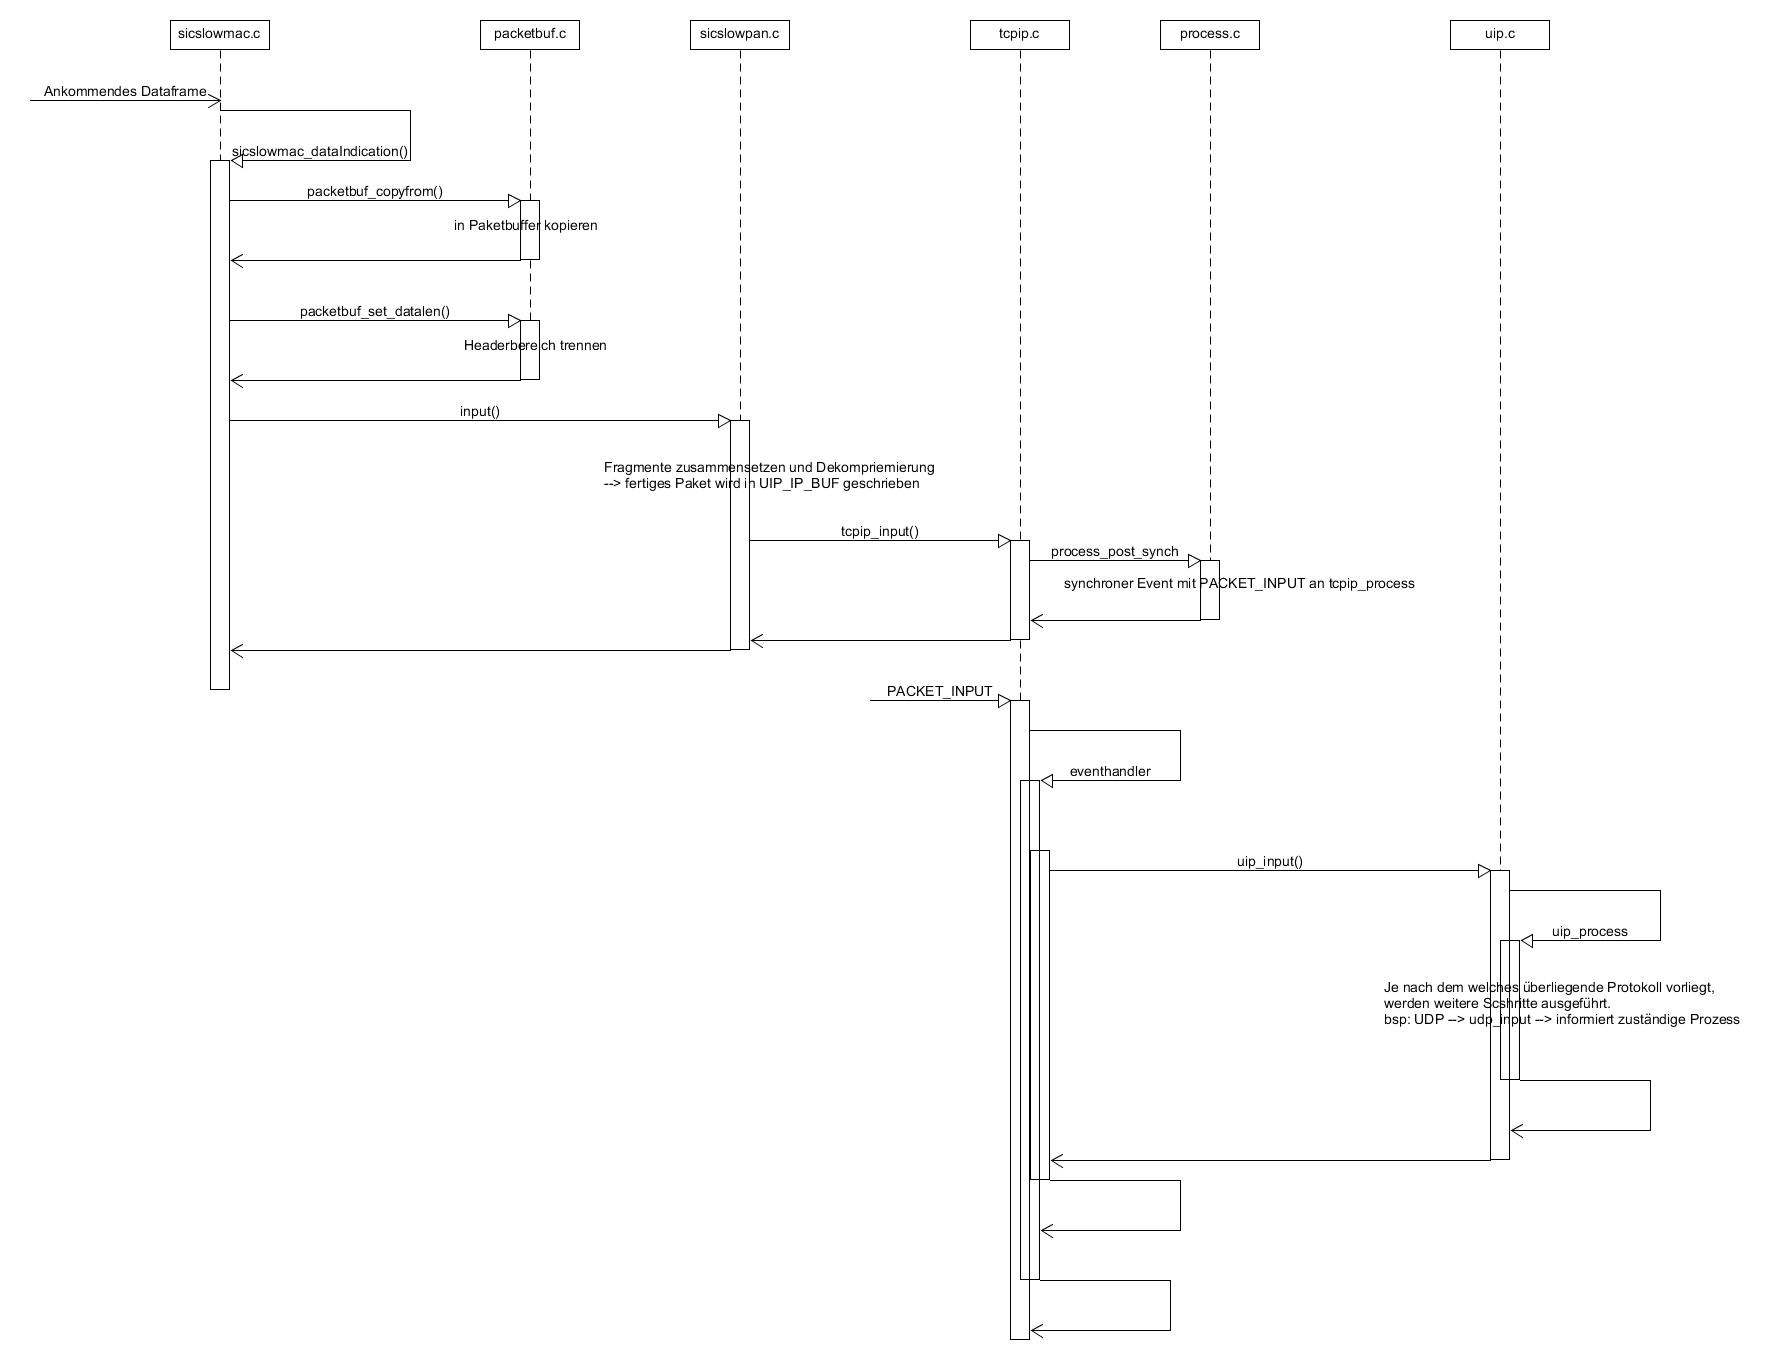
\includegraphics[scale=0.28]{Grafiken-Julian/ReceivePacket.jpg}
			\caption{Sequenzdiagramm bei Empfangen eines Pakets nach \cite{sendreceive}}
			\label{ReceivePacket}
		\end{figure}
		
	\end{itemize}
	